% -----------------------------------------------------------------
% Document class: Article
\documentclass[ a4paper, twoside, 11pt]{article}
\usepackage{../../../macros-general}
\usepackage{../../../macros-article}
% Number of the handout, quiz, exam, etc.
\newcommand{\numero}{03}
\setcounter{numero}{\numero}

% -----------------------------------------------------------------
\begin{document}
\allowdisplaybreaks

\begin{center}
\Large Mec\'anica Vectorial (MECG-1001): Trabajo Aut\'onomo \numero \\[2ex]
\small \textbf{Semestre:} 2017-2018 T\'ermino II \qquad
\textbf{Instructor:} Luis I. Reyes Castro \qquad
\textbf{Paralelo:} 09
\end{center}
\fullskip

% =============================================
\begin{problem}
\textbf{[4 Puntos]} En la siguiente armadura, encuentre las fuerzas internas en los miembros $FG$ y $FI$. Por favor, denote fuerzas de compresi\'on con signo positivo y tensi\'on con signo negativo. 

\begin{figure}[htb]
\centering
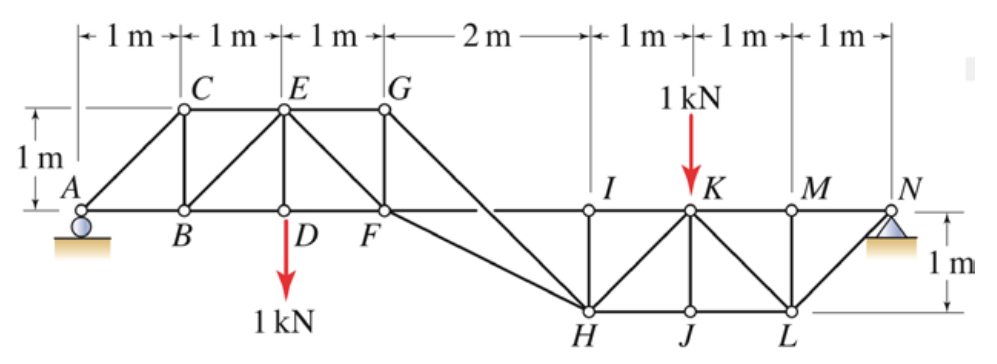
\includegraphics[width=0.64\textwidth]{problema-1.jpg}
\end{figure}

\end{problem}
\fullskip
\fullskip

% =============================================
\begin{problem}
\textbf{[4 Puntos]} Para la viga con voladizo mostrada abajo encuentre la fuerza cortante $V(x)$ y el momento flector $M(x)$ como funci\'on de la posici\'on $x \in [0,6]$. 

\begin{figure}[htb]
\centering
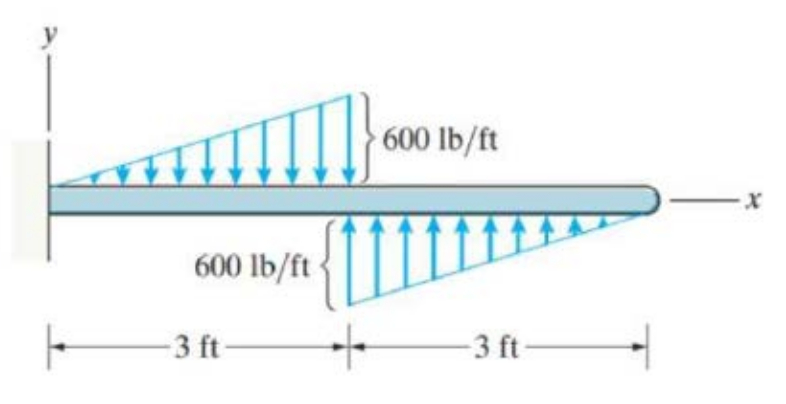
\includegraphics[width=0.56\textwidth]{problema-2.jpg}
\end{figure}

\end{problem}
\fullskip

\end{document}